\documentclass[a4paper,12pt]{article}
%\documentclass[fleqn]{article}

% ---パッケージ---
\usepackage{amsmath,amssymb}    %数式用
\usepackage{tcolorbox}   %囲み枠用(tcolorboxに変更)
\usepackage{geometry}   %余白調節
\usepackage{tikz}  % ← 図を描くためのTikZパッケージ
\geometry{margin=25mm}  %余白を少し狭く
\usetikzlibrary{decorations.pathmorphing,patterns,positioning,arrows.meta} % バネ・壁の模様
\tikzset{
  block/.style = {draw, rectangle, minimum height=2em, minimum width=3em},
  sum/.style = {draw, circle, inner sep=0pt, minimum size=5mm},
  input/.style = {coordinate},
  output/.style = {coordinate}
}
\usetikzlibrary{calc}
\usepackage{pgfplots}  % ← 追加(グラフ用)
\pgfplotsset{compat=newest} % ← 推奨設定

% --- 日本語用パッケージ ---
\usepackage{luatexja}         % 日本語表示に必要
\usepackage{luatexja-fontspec} % フォント指定用

% --- フォント指定(Overleaf標準フォント)---
\setmainjfont{IPAexMincho}  % 明朝体
%\setmainjfont{IPAexGothic}  % ゴシック体にしたい場合

% --- tcolorbox の設定 ---
\tcbset{
    colframe=black,
    colback=white,         % 本文の背景(白)
    boxrule=0.8pt,
    arc=3pt,
    outer arc=3pt,
    boxsep=4pt,
    coltitle=black,
    colbacktitle=gray!20,  % タイトルの背景(グレー)
    fonttitle=\normalsize
}

\begin{document}

\noindent
\text{制御工学Ⅰ 演習③ 解答}

\vspace{10mm}


% ---------------[1]--------------- 済
\noindent
1. 下図に示すシステムにおいて、システム全体の伝達関数を求めよ。\\
\begin{minipage}[t]{0.45\linewidth}
    (1)\\
    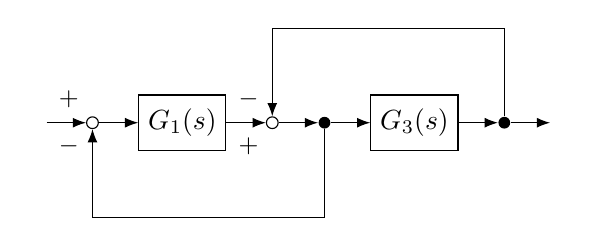
\begin{tikzpicture}[auto, node distance=0.3cm and 0.5cm, >=Latex]

        % --- 横並びのノード配置 ---
        \node at (0,0) (input) {};
        \node[circle, draw, inner sep=1.5pt, right=of input] (sum1) {};         % 合流1
        \node[block, right=of sum1] (G1) {$G_1(s)$};
        \node[circle, draw, inner sep=1.5pt, right=of G1] (sum2) {};            % 合流2
        \node[circle, fill=black, inner sep=1.5pt, right=of sum2] (branch1) {}; % 分岐1
        \node[block, right=of branch1] (G3) {$G_3(s)$};
        \node[circle, fill=black, inner sep=1.5pt, right=of G3] (branch2) {};   % 分岐2
        \node[right=of branch2] (output) {};

        % --- フィードバック座標ノード(図形なし) ---
    \coordinate (fb1) at ($(branch1)+(0,-1.2)$);
    \coordinate (fb2) at ($(branch2)+(0,1.2)$);

        % === 主系列 ===
        \draw[->] (input) -- (sum1);
        \draw[->] (sum1) -- (G1);
        \draw[->] (G1) -- (sum2);
        \draw[->] (sum2) -- (branch1);
        \draw[->] (branch1) -- (G3);
        \draw[->] (G3) -- (branch2);
        \draw[->] (branch2) -- (output);

        % === フィードバック経路 ===
        \draw[->] (branch1) |- (fb1.center) -| (sum1);
        \draw[->] (branch2) |- (fb2.center) -| (sum2);

        % --- 加算記号配置 ---
        \node at ($(sum1)+(-0.3,0.3)$) {\small $+$};
        \node at ($(sum1)+(-0.3,-0.3)$) {\small $-$};
        \node at ($(sum2)+(-0.3,0.3)$) {\small $-$};
        \node at ($(sum2)+(-0.3,-0.3)$) {\small $+$};


    \end{tikzpicture}\\

    (3)\\
    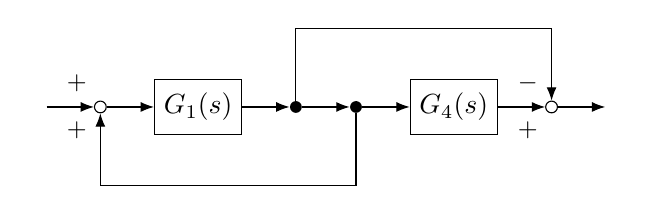
\begin{tikzpicture}[auto, node distance=0.4cm and 0.6cm, >=Latex]

            % --- 横並びノード ---
            \node at (0,0) (input) {};
            \node[circle, draw, inner sep=1.5pt, right=of input] (sum1) {};            % 合流1
            \node[block, right=of sum1] (G1) {$G_1(s)$};
            \node[circle, fill=black, inner sep=1.5pt, right=of G1] (branch1) {};      % 分岐1
            \node[circle, fill=black, inner sep=1.5pt, right=of branch1] (branch2) {}; % 分岐2
            \node[block, right=of branch2] (G4) {$G_4(s)$};
            \node[circle, draw, inner sep=1.5pt, right=of G4] (sum2) {};               % 合流2
            \node[right=of sum2] (output) {};
            
            % --- フィードバック座標 ---
            \coordinate (fb_down) at ($(branch2)+(0,-1.0)$);
            \coordinate (fb_up) at ($(branch1)+(0,1.0)$);
            
            % === 主系列 ===
            \draw[->] (input) -- (sum1);
            \draw[->] (sum1) -- (G1);
            \draw[->] (G1) -- (branch1);
            \draw[->] (branch1) -- (branch2);
            \draw[->] (branch2) -- (G4);
            \draw[->] (G4) -- (sum2);
            \draw[->] (sum2) -- (output);
            
            % === フィードバック経路 ===
            \draw[->] (branch2) |- (fb_down) -| (sum1);
            \draw[->] (branch1) |- (fb_up) -| (sum2);
            
            % --- 加算記号配置 ---
            \node at ($(sum1)+(-0.3,0.3)$) {\small $+$};
            \node at ($(sum1)+(-0.3,-0.3)$) {\small $+$};
            \node at ($(sum2)+(-0.3,0.3)$) {\small $-$};
            \node at ($(sum2)+(-0.3,-0.3)$) {\small $+$};
            
    \end{tikzpicture}
\end{minipage}
\hfill
\begin{minipage}[t]{0.45\linewidth}
    (2)\\
    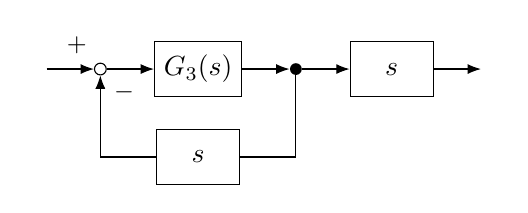
\begin{tikzpicture}[auto, node distance=0.4cm and 0.6cm, >=Latex]

        % --- 横並びの主系列ノード ---
        \node at (0,0) (input) {};
        \node[circle, draw, inner sep=1.5pt, right=of input] (sum) {};
        \node[block, right=of sum] (G3) {$G_3(s)$};
        \node[circle, fill=black, inner sep=1.5pt, right=of G3] (branch) {};
        \node[block, right=of branch] (s1) {$s$};
        \node[right=of s1] (output) {};
        
        % --- 下の s ノード ---
        \node[block, below=of G3] (s2) {$s$};
        
        % === 主系列 ===
        \draw[->] (input) -- (sum);
        \draw[->] (sum) -- (G3);
        \draw[->] (G3) -- (branch);
        \draw[->] (branch) -- (s1);
        \draw[->] (s1) -- (output);
        
        % === フィードバック経路(下) ===
        \draw[->] (branch) |- (s2) -| (sum);
        
        % --- 加算記号配置 ---
        \node at ($(sum)+(-0.3,0.3)$) {\small $+$};
        \node at ($(sum)+(0.3,-0.3)$) {\small $-$};
        
    \end{tikzpicture}\\

    (4)\\
    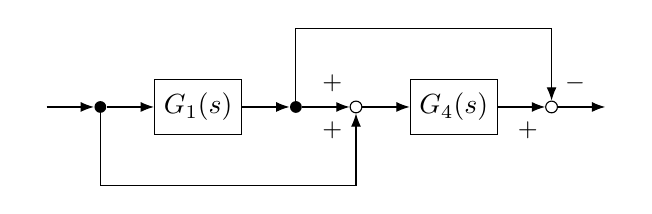
\begin{tikzpicture}[auto, node distance=0.4cm and 0.6cm, >=Latex]

        % --- 横並びノード(sum1 と branch2 の位置を交換) ---
        \node at (0,0) (input) {};
        \node[circle, fill=black, inner sep=1.5pt, right=of input] (branch2) {};     % ← 分岐2
        \node[block, right=of branch2] (G1) {$G_1(s)$};
        \node[circle, fill=black, inner sep=1.5pt, right=of G1] (branch1) {};        % 分岐1
        \node[circle, draw, inner sep=1.5pt, right=of branch1] (sum1) {};            % ← 合流1
        \node[block, right=of sum1] (G4) {$G_4(s)$};
        \node[circle, draw, inner sep=1.5pt, right=of G4] (sum2) {};                 % 合流2
        \node[right=of sum2] (output) {};
        
        % --- フィードバック座標 ---
        \coordinate (fb_down) at ($(branch2)+(0,-1.0)$);
        \coordinate (fb_up) at ($(branch1)+(0,1.0)$);
        
        % === 主系列 ===
        \draw[->] (input) -- (branch2);
        \draw[->] (branch2) -- (G1);
        \draw[->] (G1) -- (branch1);
        \draw[->] (branch1) -- (sum1);
        \draw[->] (sum1) -- (G4);
        \draw[->] (G4) -- (sum2);
        \draw[->] (sum2) -- (output);
        
        % === フィードバック経路 ===
        \draw[->] (branch2) |- (fb_down) -| (sum1);
        \draw[->] (branch1) |- (fb_up) -| (sum2);
        
        % --- 加算記号配置 ---
        \node at ($(sum1)+(-0.3,0.3)$) {\small $+$};
        \node at ($(sum1)+(-0.3,-0.3)$) {\small $+$};
        \node at ($(sum2)+(-0.3,-0.3)$) {\small $+$};
        \node at ($(sum2)+(0.3,0.3)$) {\small $-$};
        
    \end{tikzpicture}
\end{minipage}\\


\begin{tcolorbox}[title={1. (1)
    \vspace{-6mm}
    \begin{center}
        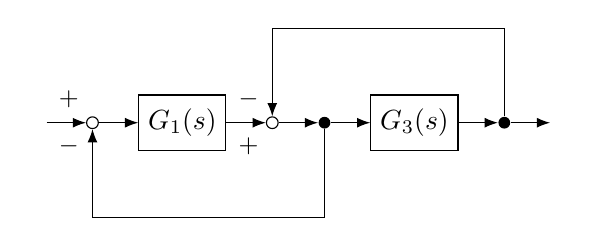
\begin{tikzpicture}[auto, node distance=0.3cm and 0.5cm, >=Latex]

        % --- 横並びのノード配置 ---
        \node at (0,0) (input) {};
        \node[circle, draw, inner sep=1.5pt, right=of input] (sum1) {};         % 合流1
        \node[block, right=of sum1] (G1) {$G_1(s)$};
        \node[circle, draw, inner sep=1.5pt, right=of G1] (sum2) {};            % 合流2
        \node[circle, fill=black, inner sep=1.5pt, right=of sum2] (branch1) {}; % 分岐1
        \node[block, right=of branch1] (G3) {$G_3(s)$};
        \node[circle, fill=black, inner sep=1.5pt, right=of G3] (branch2) {};   % 分岐2
        \node[right=of branch2] (output) {};

        % --- フィードバック座標ノード(図形なし) ---
    \coordinate (fb1) at ($(branch1)+(0,-1.2)$);
    \coordinate (fb2) at ($(branch2)+(0,1.2)$);

        % === 主系列 ===
        \draw[->] (input) -- (sum1);
        \draw[->] (sum1) -- (G1);
        \draw[->] (G1) -- (sum2);
        \draw[->] (sum2) -- (branch1);
        \draw[->] (branch1) -- (G3);
        \draw[->] (G3) -- (branch2);
        \draw[->] (branch2) -- (output);

        % === フィードバック経路 ===
        \draw[->] (branch1) |- (fb1.center) -| (sum1);
        \draw[->] (branch2) |- (fb2.center) -| (sum2);

        % --- 加算記号配置 ---
        \node at ($(sum1)+(-0.3,0.3)$) {\small $+$};
        \node at ($(sum1)+(-0.3,-0.3)$) {\small $-$};
        \node at ($(sum2)+(-0.3,0.3)$) {\small $-$};
        \node at ($(sum2)+(-0.3,-0.3)$) {\small $+$};


    \end{tikzpicture}
    \end{center}  }]

\begin{center}
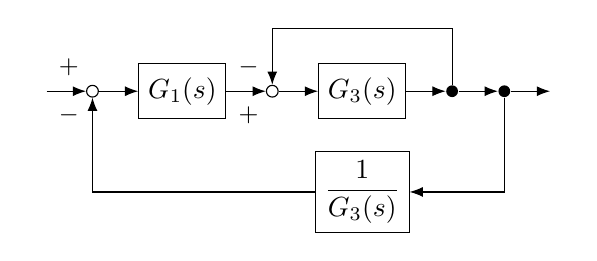
\begin{tikzpicture}[auto, node distance=0.3cm and 0.5cm, >=Latex]

  % --- 横並びノード配置 ---
  \node at (0,0) (input) {};
  \node[circle, draw, inner sep=1.5pt, right=of input] (sum1) {};               % 合流1
  \node[block, right=of sum1] (G1) {$G_1(s)$};
  \node[circle, draw, inner sep=1.5pt, right=of G1] (sum2) {};                  % 合流2
  \node[block, right=of sum2] (G3) {$G_3(s)$};
  \node[circle, fill=black, inner sep=1.5pt, right=of G3] (branch2) {};         % 分岐2(元の位置)
  \node[circle, fill=black, inner sep=1.5pt, right=of branch2] (branch1) {};    % 分岐1(右に移動)
  \node[right=of branch1] (output) {};

  % --- 1/G3ノード(下段) ---
  \node[block, below=0.4cm of G3] (invG3) {$\dfrac{1}{G_3(s)}$};

  % --- フィードバック座標(branch2 → sum2) ---
  \coordinate (fb2) at ($(branch2)+(0,0.8)$);

  % === 主系列 ===
  \draw[->] (input) -- (sum1);
  \draw[->] (sum1) -- (G1);
  \draw[->] (G1) -- (sum2);
  \draw[->] (sum2) -- (G3);
  \draw[->] (G3) -- (branch2);
  \draw[->] (branch2) -- (branch1);
  \draw[->] (branch1) -- (output);

  % === フィードバックルート1(branch1 → 1/G3 → sum1)===
  \draw[->] (branch1) |- (invG3);
  \draw[->] (invG3) -| (sum1);

  % === フィードバックルート2(branch2 → sum2)===
  \draw[->] (branch2) |- (fb2) -| (sum2);

  % --- 加算記号配置 ---
  \node at ($(sum1)+(-0.3,0.3)$) {\small $+$};
  \node at ($(sum1)+(-0.3,-0.3)$) {\small $-$};
  \node at ($(sum2)+(-0.3,0.3)$) {\small $-$};
  \node at ($(sum2)+(-0.3,-0.3)$) {\small $+$};

\end{tikzpicture}

\vspace{2mm}
    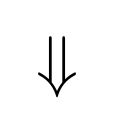
\begin{tikzpicture}
    \node {\Huge$\Downarrow$};
    \end{tikzpicture}
\vspace{2mm}



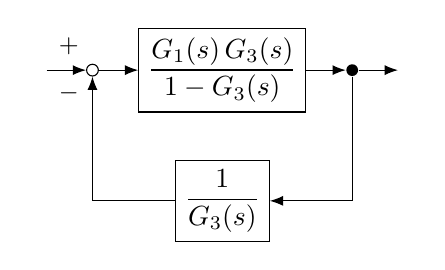
\begin{tikzpicture}[auto, node distance=0.3cm and 0.5cm, >=Latex]

  % --- 横並びノード配置 ---
  \node at (0,0) (input) {};
  \node[circle, draw, inner sep=1.5pt, right=of input] (sum1) {};                     % 合流点
  \node[block, right=of sum1] (G13series) {$\dfrac{G_1(s)\,G_3(s)}{1 - G_3(s)}$};     % 直列合成済
  \node[circle, fill=black, inner sep=1.5pt, right=of G13series] (branch1) {};        % 分岐点
  \node[right=of branch1] (output) {};

  % --- フィードバック用ノード ---
  \node[block, below=0.6cm of G13series] (invG3) {$\dfrac{1}{G_3(s)}$};

  % --- 主系列 ---
  \draw[->] (input) -- (sum1);
  \draw[->] (sum1) -- (G13series);
  \draw[->] (G13series) -- (branch1);
  \draw[->] (branch1) -- (output);

  % --- フィードバック(branch1 → 1/G3 → sum1) ---
  \draw[->] (branch1) |- (invG3);
  \draw[->] (invG3) -| (sum1);

  % --- 加算記号 ---
  \node at ($(sum1)+(-0.3,0.3)$) {\small $+$};
  \node at ($(sum1)+(-0.3,-0.3)$) {\small $-$};

\end{tikzpicture}

\vspace{2mm}
    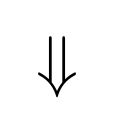
\begin{tikzpicture}
    \node {\Huge$\Downarrow$};
    \end{tikzpicture}
\vspace{2mm}


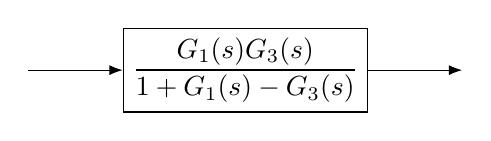
\begin{tikzpicture}[auto, node distance=1.5cm and 1.2cm, >=Latex]

  % --- ノード構成 ---
  \node[input] (input) {};
  \node[block, right=of input] (Gfinal) {$\dfrac{G_1(s) G_3(s)}{1 + G_1(s) - G_3(s)}$};
  \node[output, right=of Gfinal] (output) {};

  % --- 線描画 ---
  \draw[->] (input) -- (Gfinal);
  \draw[->] (Gfinal) -- (output);

\end{tikzpicture}




\end{center}

\vspace{-2mm}
よって、システム全体の伝達関数\(G_{All}(s)\)は
\vspace{-4mm}
\[
G_{All}(s) = \dfrac{G_1(s) G_3(s)}{1 + G_1(s) - G_3(s)}
\]


\end{tcolorbox}

\begin{tcolorbox}[title={1. (2)
    \vspace{-6mm}
    \begin{center}
        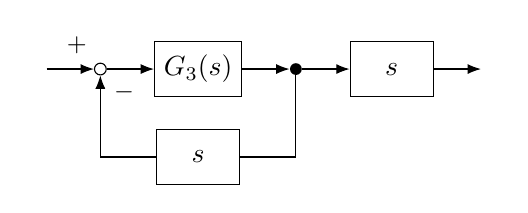
\begin{tikzpicture}[auto, node distance=0.4cm and 0.6cm, >=Latex]

        % --- 横並びの主系列ノード ---
        \node at (0,0) (input) {};
        \node[circle, draw, inner sep=1.5pt, right=of input] (sum) {};
        \node[block, right=of sum] (G3) {$G_3(s)$};
        \node[circle, fill=black, inner sep=1.5pt, right=of G3] (branch) {};
        \node[block, right=of branch] (s1) {$s$};
        \node[right=of s1] (output) {};
        
        % --- 下の s ノード ---
        \node[block, below=of G3] (s2) {$s$};
        
        % === 主系列 ===
        \draw[->] (input) -- (sum);
        \draw[->] (sum) -- (G3);
        \draw[->] (G3) -- (branch);
        \draw[->] (branch) -- (s1);
        \draw[->] (s1) -- (output);
        
        % === フィードバック経路(下) ===
        \draw[->] (branch) |- (s2) -| (sum);
        
        % --- 加算記号配置 ---
        \node at ($(sum)+(-0.3,0.3)$) {\small $+$};
        \node at ($(sum)+(0.3,-0.3)$) {\small $-$};
        
        \end{tikzpicture}
    \end{center} }]

    \begin{center}
        
        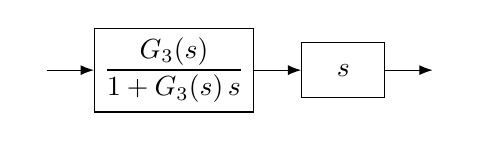
\begin{tikzpicture}[auto, node distance=0.4cm and 0.6cm, >=Latex]

        % --- ノード配置(フィードバック合成済・合流と分岐削除) ---
        \node at (0,0) (input) {};
        \node[block, right=of input] (Gfb) {$\dfrac{G_3(s)}{1 + G_3(s)\,s}$};
        \node[block, right=of Gfb] (s1) {$s$};
        \node[right=of s1] (output) {};

        % === 主系列 ===
        \draw[->] (input) -- (Gfb);
        \draw[->] (Gfb) -- (s1);
        \draw[->] (s1) -- (output);

        \end{tikzpicture}

        \vspace{2mm}
            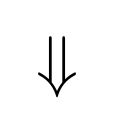
\begin{tikzpicture}
            \node {\Huge$\Downarrow$};
            \end{tikzpicture}
        \vspace{2mm}


        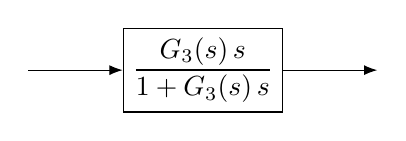
\begin{tikzpicture}[auto, node distance=1.5cm and 1.2cm, >=Latex]

        % --- ノード構成(完全合成) ---
        \node[input] (input) {};
        \node[block, right=of input] (Gfinal) {$\dfrac{G_3(s)\,s}{1 + G_3(s)\,s}$};
        \node[output, right=of Gfinal] (output) {};

        % --- 線描画 ---
        \draw[->] (input) -- (Gfinal);
        \draw[->] (Gfinal) -- (output);

        \end{tikzpicture}

    \end{center}

    \vspace{-2mm}
よって、システム全体の伝達関数\(G_{All}(s)\)は
\vspace{-4mm}
\[
G_{All}(s) = \dfrac{G_3(s)\,s}{1 + G_3(s)\,s}
\]

\end{tcolorbox}

\begin{tcolorbox}[title={1. (3)
    \vspace{-6mm}
    \begin{center}
        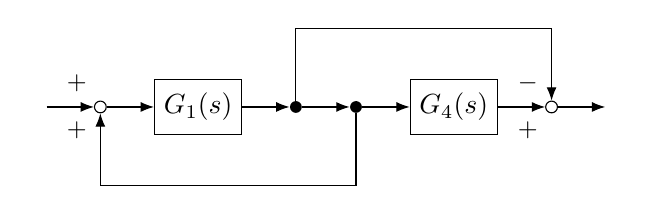
\begin{tikzpicture}[auto, node distance=0.4cm and 0.6cm, >=Latex]

            % --- 横並びノード ---
            \node at (0,0) (input) {};
            \node[circle, draw, inner sep=1.5pt, right=of input] (sum1) {};            % 合流1
            \node[block, right=of sum1] (G1) {$G_1(s)$};
            \node[circle, fill=black, inner sep=1.5pt, right=of G1] (branch1) {};      % 分岐1
            \node[circle, fill=black, inner sep=1.5pt, right=of branch1] (branch2) {}; % 分岐2
            \node[block, right=of branch2] (G4) {$G_4(s)$};
            \node[circle, draw, inner sep=1.5pt, right=of G4] (sum2) {};               % 合流2
            \node[right=of sum2] (output) {};
            
            % --- フィードバック座標 ---
            \coordinate (fb_down) at ($(branch2)+(0,-1.0)$);
            \coordinate (fb_up) at ($(branch1)+(0,1.0)$);
            
            % === 主系列 ===
            \draw[->] (input) -- (sum1);
            \draw[->] (sum1) -- (G1);
            \draw[->] (G1) -- (branch1);
            \draw[->] (branch1) -- (branch2);
            \draw[->] (branch2) -- (G4);
            \draw[->] (G4) -- (sum2);
            \draw[->] (sum2) -- (output);
            
            % === フィードバック経路 ===
            \draw[->] (branch2) |- (fb_down) -| (sum1);
            \draw[->] (branch1) |- (fb_up) -| (sum2);
            
            % --- 加算記号配置 ---
            \node at ($(sum1)+(-0.3,0.3)$) {\small $+$};
            \node at ($(sum1)+(-0.3,-0.3)$) {\small $+$};
            \node at ($(sum2)+(-0.3,0.3)$) {\small $-$};
            \node at ($(sum2)+(-0.3,-0.3)$) {\small $+$};
            
        \end{tikzpicture}
    \end{center}  }]

    \begin{center}
        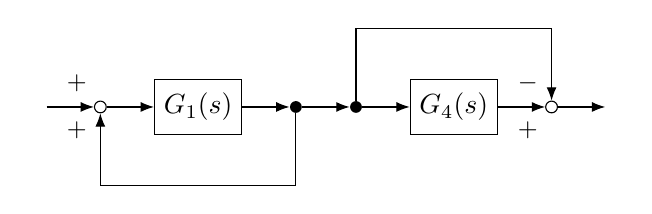
\begin{tikzpicture}[auto, node distance=0.4cm and 0.6cm, >=Latex]

        % --- 横並びノード(分岐1と分岐2の位置を入れ替え) ---
        \node at (0,0) (input) {};
        \node[circle, draw, inner sep=1.5pt, right=of input] (sum1) {};                  % 合流1
        \node[block, right=of sum1] (G1) {$G_1(s)$};
        \node[circle, fill=black, inner sep=1.5pt, right=of G1] (branch2) {};            % 分岐2(元:分岐1)
        \node[circle, fill=black, inner sep=1.5pt, right=of branch2] (branch1) {};       % 分岐1(元:分岐2)
        \node[block, right=of branch1] (G4) {$G_4(s)$};
        \node[circle, draw, inner sep=1.5pt, right=of G4] (sum2) {};                     % 合流2
        \node[right=of sum2] (output) {};

        % --- フィードバック座標 ---
        \coordinate (fb_down) at ($(branch2)+(0,-1.0)$);
        \coordinate (fb_up) at ($(branch1)+(0,1.0)$);

        % === 主系列 ===
        \draw[->] (input) -- (sum1);
        \draw[->] (sum1) -- (G1);
        \draw[->] (G1) -- (branch2);
        \draw[->] (branch2) -- (branch1);
        \draw[->] (branch1) -- (G4);
        \draw[->] (G4) -- (sum2);
        \draw[->] (sum2) -- (output);

        % === フィードバック経路(分岐位置入れ替えに従って接続) ===
        \draw[->] (branch2) |- (fb_down) -| (sum1);
        \draw[->] (branch1) |- (fb_up) -| (sum2);

        % --- 加算記号配置 ---
        \node at ($(sum1)+(-0.3,0.3)$) {\small $+$};
        \node at ($(sum1)+(-0.3,-0.3)$) {\small $+$};
        \node at ($(sum2)+(-0.3,0.3)$) {\small $-$};
        \node at ($(sum2)+(-0.3,-0.3)$) {\small $+$};

        \end{tikzpicture}

        \vspace{2mm}
            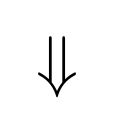
\begin{tikzpicture}
            \node {\Huge$\Downarrow$};
            \end{tikzpicture}
        \vspace{2mm}

        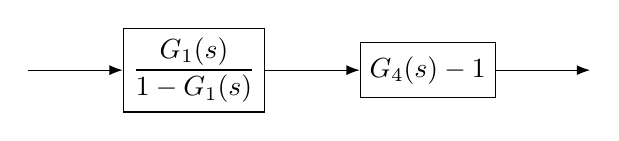
\begin{tikzpicture}[auto, node distance=1.8cm and 1.2cm, >=Latex]

        % --- 合成済みノード構成(G1と下段フィードバック、G4とsum2 合成済) ---
        \node[input] (input) {};
        \node[block, right=of input] (Gleft) {$\dfrac{G_1(s)}{1 - G_1(s)}$};          % G1と正帰還合成
        \node[block, right=of Gleft] (Gright) {$G_4(s) - 1$};                         % G4とsum2(−合流)合成
        \node[output, right=of Gright] (output) {};

        % --- 線描画 ---
        \draw[->] (input) -- (Gleft);
        \draw[->] (Gleft) -- (Gright);
        \draw[->] (Gright) -- (output);

        \end{tikzpicture}

        \vspace{2mm}
            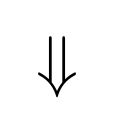
\begin{tikzpicture}
            \node {\Huge$\Downarrow$};
            \end{tikzpicture}
        \vspace{2mm}

        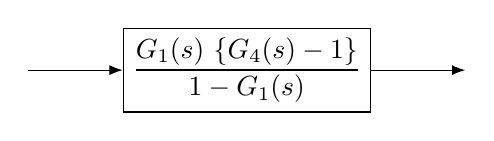
\begin{tikzpicture}[auto, node distance=2.0cm and 1.2cm, >=Latex]

        % --- 合成済みノード構成(完全合成) ---
        \node[input] (input) {};
        \node[block, right=of input] (Gfinal) 
            {$\displaystyle \frac{G_1(s)\,\left\{G_4(s) - 1\right\}}{1 - G_1(s)}$};
        \node[output, right=of Gfinal] (output) {};

        % --- 線描画 ---
        \draw[->] (input) -- (Gfinal);
        \draw[->] (Gfinal) -- (output);

        \end{tikzpicture}

    \end{center}
    よって、システム全体の伝達関数\(G_{All}(s)\)は
\[
G_{All}(s) = \dfrac{G_1(s)\,\left\{G_4(s) - 1\right\}}{1 - G_1(s)}
\]
\end{tcolorbox}

\begin{tcolorbox}[title={1. (4)
    \vspace{-6mm}
    \begin{center}
        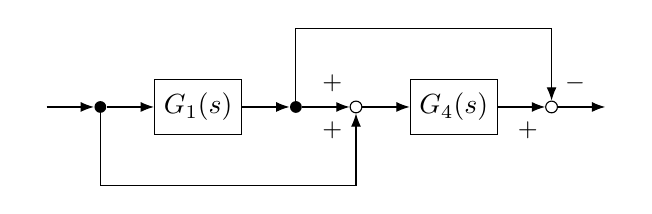
\begin{tikzpicture}[auto, node distance=0.4cm and 0.6cm, >=Latex]

        % --- 横並びノード(sum1 と branch2 の位置を交換) ---
        \node at (0,0) (input) {};
        \node[circle, fill=black, inner sep=1.5pt, right=of input] (branch2) {};     % ← 分岐2
        \node[block, right=of branch2] (G1) {$G_1(s)$};
        \node[circle, fill=black, inner sep=1.5pt, right=of G1] (branch1) {};        % 分岐1
        \node[circle, draw, inner sep=1.5pt, right=of branch1] (sum1) {};            % ← 合流1
        \node[block, right=of sum1] (G4) {$G_4(s)$};
        \node[circle, draw, inner sep=1.5pt, right=of G4] (sum2) {};                 % 合流2
        \node[right=of sum2] (output) {};
        
        % --- フィードバック座標 ---
        \coordinate (fb_down) at ($(branch2)+(0,-1.0)$);
        \coordinate (fb_up) at ($(branch1)+(0,1.0)$);
        
        % === 主系列 ===
        \draw[->] (input) -- (branch2);
        \draw[->] (branch2) -- (G1);
        \draw[->] (G1) -- (branch1);
        \draw[->] (branch1) -- (sum1);
        \draw[->] (sum1) -- (G4);
        \draw[->] (G4) -- (sum2);
        \draw[->] (sum2) -- (output);
        
        % === フィードバック経路 ===
        \draw[->] (branch2) |- (fb_down) -| (sum1);
        \draw[->] (branch1) |- (fb_up) -| (sum2);
        
        % --- 加算記号配置 ---
        \node at ($(sum1)+(-0.3,0.3)$) {\small $+$};
        \node at ($(sum1)+(-0.3,-0.3)$) {\small $+$};
        \node at ($(sum2)+(-0.3,-0.3)$) {\small $+$};
        \node at ($(sum2)+(0.3,0.3)$) {\small $-$};
        
        \end{tikzpicture}
    \end{center}  }]

    \begin{center}
    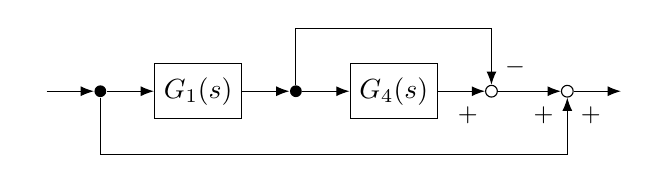
\begin{tikzpicture}[auto, node distance=0.4cm and 0.6cm, >=Latex]

    % --- 横並びノード(sum1 を sum2 の右へ移動) ---
    \node at (0,0) (input) {};
    \node[circle, fill=black, inner sep=1.5pt, right=of input] (branch2) {};           % 分岐2
    \node[block, right=of branch2] (G1) {$G_1(s)$};
    \node[circle, fill=black, inner sep=1.5pt, right=of G1] (branch1) {};              % 分岐1
    \node[block, right=of branch1] (G4) {$G_4(s)$};
    \node[circle, draw, inner sep=1.5pt, right=of G4] (sum2) {};                       % 合流2(そのまま)
    \node[circle, draw, inner sep=1.5pt, right=0.8cm of sum2] (sum1) {};                     % 合流1(移動後)
    \node[right=of sum1] (output) {};

    % --- フィードバック座標 ---
    \coordinate (fb_down) at ($(branch2)+(0,-0.8)$);
    \coordinate (fb_up) at ($(branch1)+(0,0.8)$);

    % === 主系列 ===
    \draw[->] (input) -- (branch2);
    \draw[->] (branch2) -- (G1);
    \draw[->] (G1) -- (branch1);
    \draw[->] (branch1) -- (G4);
    \draw[->] (G4) -- (sum2);
    \draw[->] (sum2) -- (sum1);
    \draw[->] (sum1) -- (output);

    % === フィードバック経路(branch2 → sum1)、位置変更に対応 ===
    \draw[->] (branch2) |- (fb_down) -| (sum1);
    \draw[->] (branch1) |- (fb_up) -| (sum2);

    % --- 加算記号配置 ---
    \node at ($(sum1)+(0.3,-0.3)$) {\small $+$};
    \node at ($(sum1)+(-0.3,-0.3)$) {\small $+$};
    \node at ($(sum2)+(0.3,0.3)$) {\small $-$};
    \node at ($(sum2)+(-0.3,-0.3)$) {\small $+$};

    \end{tikzpicture}

    \vspace{2mm}
        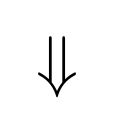
\begin{tikzpicture}
        \node {\Huge$\Downarrow$};
        \end{tikzpicture}
    \vspace{2mm}

    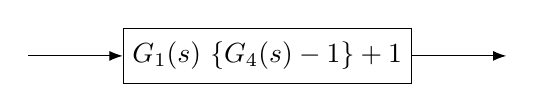
\begin{tikzpicture}[auto, node distance=2.0cm and 1.2cm, >=Latex]

    % --- 合成済みノード構成(完全伝達関数) ---
    \node[input] (input) {};
    \node[block, right=of input] (Gfinal) 
        {$\displaystyle G_1(s)\,\left\{G_4(s) - 1\right\} + 1$};
    \node[output, right=of Gfinal] (output) {};

    % --- 線描画 ---
    \draw[->] (input) -- (Gfinal);
    \draw[->] (Gfinal) -- (output);

    \end{tikzpicture}

    \end{center}
\vspace{-4mm}
よって、システム全体の伝達関数\(G_{All}(s)\)は
\vspace{-2mm}
\[
G_{All}(s) = G_1(s)\,\left\{G_4(s) - 1\right\} + 1
\]
\end{tcolorbox}


% ---------------[2]--------------- 済
\begin{tcolorbox}[title={2.\quad \(\ddot{x}(t) - \sin(\omega t) = 0\) を解け。ただし、初期値はすべて0とする。
    }]
    \quad 両辺にラプラス変換を施すと,
    \vspace{-3mm}
    \begin{align*}
        &\qquad \mathcal{L}\left[ \ddot{x}(t) - \sin(\omega t) \right] 
        = 0 \\
        &\Leftrightarrow \left\{ s^2 X(s) - sx(0) - \dot{x}(0) \right\}
        - \frac{\omega}{s^2 + \omega^2}
        = 0  \\
        &\Leftrightarrow X(s) = \frac{\omega}{s^2(s^2 + \omega^2)}  \\
        &\Leftrightarrow X(s) = \frac{1}{\omega}\left\{\frac{1}{s^2} - \frac{1}{s^2 + \omega^2} \right\} 
    \end{align*}
    \vspace{-4mm}
    \quad 両辺にラプラス逆変換を施すと,
    \begin{align*}
    &\qquad \mathcal{L}^{-1} \left[ X(s) \right] 
    = \mathcal{L}^{-1} \left[ \frac{1}{\omega}\left\{\frac{1}{s^2} - \frac{1}{\omega} \frac{\omega}{s^2 + \omega^2} \right\}  \right] \\
    &\Leftrightarrow x(t) = \frac{1}{\omega} \left( t - \frac{1}{\omega} \sin \omega t \right)
    \end{align*}

\end{tcolorbox}

% ---------------[3]--------------- 済
\begin{tcolorbox}[title={3. 伝達関数\(\dfrac{s+1}{s^2+2s+4}\)のラプラス逆変換を行え。
    }]
    \vspace{-5mm}
\begin{align*}
    &\qquad G(s) =\frac{s+1}{s^2+2s+4}  \\
    &\Leftrightarrow G(s) =\frac{s + 1}{ ( s + 1 )^2+ 3} 
\end{align*}

\quad 両辺にラプラス逆変換を施すと,
\vspace{-3mm}
\begin{align*}
    &\qquad \mathcal{L}^{-1} \left[ G(s) \right] 
    =\mathcal{L}^{-1} \left[ \frac{s + 1}{ ( s + 1 )^2+ 3}  \right] \\
    &\Leftrightarrow g(t) = e^{-t} \cos (\sqrt{3} t)   
\end{align*}

\end{tcolorbox}



% ---------------[4]---------------
\noindent
\begin{minipage}[t]{0.005\linewidth}
    4.
\end{minipage}
\hfill
\begin{minipage}[t]{0.595\linewidth}
右図に示す系について、入力を変位\(x_1(t)\)、出力を変位\(x_2(t)\)としたとき、
次の問いに答えよ。なお、\(m\)は質量[kg]、\(d\)は粘性係数[Ns/m]、
\(k_1\)、\(k_2\)はバネ[N/m] 
とし、初期状態において系は静止しているとする。  
\end{minipage}
\hfill
\begin{minipage}[t]{0.35\linewidth}
    \vspace{-6mm}
    \begin{center}
        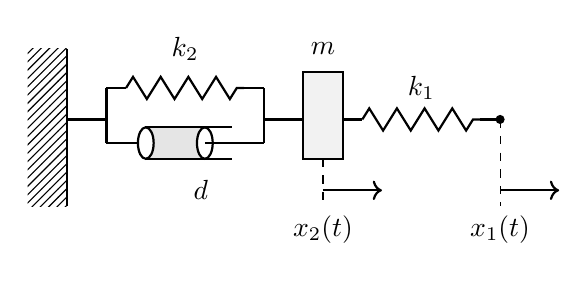
\begin{tikzpicture}[scale=1.0]
          % 固定壁
          \fill[pattern=north east lines] (-1,0,0) rectangle (-0.5,2);
          \draw[thick] (-0.5,0) -- (-0.5,2);
      
          %接続部1
          \draw[thick] (-0.5,1.1) -- (0,1.1);
          \draw[thick] (0,0.8) -- (0,1.5);
        
          % バネ2
          \draw[thick] (0,1.5) -- (0.25,1.5);
          \draw[thick, decorate, decoration={zigzag, segment length=10, amplitude=4}] (0.25,1.5) -- (1.75,1.5);
          \draw[thick] (1.75,1.5) -- (2.0,1.5);
          \node at (1.0,2.0) {$k_2$};
        
          % ダンパー(シリンダー形式)
          \draw[thick] (0,0.8) -- (0.5,0.8); % 棒
          \draw[thick, fill=gray!20] (0.5,0.6) rectangle (1.25,1.0); % 筒の側面
          \draw[thick] (1.25,1.0) -- (1.60,1.0); % 筒の上
          \draw[thick] (1.25,0.6) -- (1.60,0.6); % 筒の下
          \draw[thick, fill=white] (0.5,0.8) ellipse (0.1 and 0.2); % 左端面
          \draw[thick, fill=white] (1.25,0.8) ellipse (0.1 and 0.2); % 右端面
          \draw[thick] (1.25,0.8) -- (2.0,0.8); % ピストン棒
          \node at (1.2,0.2) {$d$};
      
          %接続部2
          \draw[thick] (2.0,0.8) -- (2.0,1.5);
          \draw[thick] (2.0,1.1) -- (2.5,1.1);
        
          % 質量M
          \draw[thick, fill=gray!10] (2.5,0.6) rectangle (3.0,1.7);
          \node at (2.75,2.0) {$m$};
      
          % バネ1
          \draw[thick] (3.0,1.1) -- (3.25,1.1);
          \draw[thick, decorate, decoration={zigzag, segment length=10, amplitude=4}] (3.25,1.1) -- (4.75,1.1);
          \draw[thick] (4.75,1.1) -- (5.0,1.1);
          \node at (4.0,1.5) {$k_1$};
      
          % 丸
          \draw[fill] (5,1.1) circle (0.05);
      
        
          % 座標x1
          \draw[->, thick] (5,0.2) -- (5.75,0.2);
          \node at (5,-0.3) {$x_1(t)$};
          \draw[dashed] (5,1.1) -- (5,0);
      
          % 座標x2
          \draw[->, thick] (2.75,0.2) -- (3.5,0.2);
          \node at (2.75,-0.3) {$x_2(t)$};
          \draw[dashed] (2.75,0.6) -- (2.75,0);
        
        \end{tikzpicture}
    \end{center}
\end{minipage}\\

\indent
(1)この図によって示されるシステムの運動方程式と伝達関数を求めよ。\\

\indent
(2)\(m=1,d=4,k_1=1,k_2=2\)とし、インパルス応答、ステップ応答をそれぞれ求\\
\indent \quad めよ。\\

\indent
(3)\(m=1,d=2,k_1=3,k_2=2\)とし、ステップ応答を求めよ。\\

\indent
(4)\(m=1,d=2,k_1=1,k_2=0\)とし、ステップ応答を求めよ。\\

\indent
(5)\(m=1,d=0,k_1=1,k_2=2\)とし、ステップ応答を求めよ。\\

\indent
(6)\(m=1,d=0,k_1=2,k_2=1\)とし、入力変位\(x_1(t)=\sin(t)\)を与えたときの応答を求
\indent \quad めよ。\\

\indent
(7)\(m=1,d=2,k_1=1,k_2=1\)とし、入力変位\(x_1(t)=\sin(2t)\)を与えたときの応答を
\indent \quad 求めよ。\\

% ---------------[4(1)]--------------- 済
\begin{tcolorbox}[title={4. (1)この図によって示されるシステムの運動方程式と伝達関数を求めよ。 
    }]

    \(x(t)\)に関する運動方程式は
    \begin{align*}
        &\qquad m\ddot{x}_2 =-k_2 x_2 - d \dot{x}_2 - k_1 \left(x_2 - x_1\right) \\
    \end{align*}
    また伝達関数は
    \begin{align*}
        &\qquad m\ddot{x}_2 +  d \dot{x}_2 + \left(k_1+k_2\right) x_2
        = k_1 x_1 \\
        &\therefore \quad \mathcal{L} \left[ m\ddot{x}_2 +  d \dot{x}_2 + \left(k_1+k_2\right) x_2\right] 
        =\mathcal{L} \left[ k_1 x_1 \right] \\
        &\therefore \quad \left\{m s^2 + d s + \left(k_1+k_2\right) \right\}\,X_2(s) = k_1 X_1(s) \quad [\because \dot{x}(0)=x(0)=0 ]\\
        &\therefore \quad G(s) \;=\;\frac{X_2(s)}{X_1(s)}
        \;=\;\frac{k_1}{m s^2 + d s + \left(k_1 + k_2\right)}
    \end{align*}

\end{tcolorbox}

% ---------------[4(2)]--------------- 済
\begin{tcolorbox}[title={4. (2)\(m=1,d=4,k_1=1,k_2=2\)とし、インパルス応答、ステップ応答をそれぞれ\\
\indent \quad 求めよ。}]

    (\uppercase\expandafter{\romannumeral 1})インパルス応答 \\
    パラメータを代入し、インパルス入力のラプラス変換は\(F(s)=1\)なので
    \vspace{-2mm}
    \begin{align*}
        &\qquad G(s) = \frac{1}{s^2 + 4 s + 3 } \\
        &\therefore \quad X(s) = G(s) F(s) = \frac{1}{(s+1)(s+3)} \\
        &\therefore \quad X(s) = \frac{1}{2} \left( \frac{1}{s+1} + \frac{-1}{s+3} \right)\\
        &\therefore \quad \mathcal{L}^{-1} \left[ X(s)\right] 
        =\frac{1}{2} \left\{ \mathcal{L}^{-1} \left[\frac{1}{s+1}\right] 
        + \mathcal{L}^{-1} \left[\frac{-1}{s+3}\right] \right\}\\
        &\therefore \quad x(t) = \frac{1}{2}\left(e^{-t} - e^{-3t} \right)
    \end{align*}

    (\uppercase\expandafter{\romannumeral 2})ステップ応答 \\
    パラメータを代入し、ステップ入力のラプラス変換は\(F(s)=\dfrac{1}{s}\)なので
    \vspace{-2mm}
    \begin{align*}
        &\qquad G(s) = \frac{1}{s^2 + 4 s + 3 } \\
        &\therefore \quad X(s) = G(s) F(s) = \frac{1}{s(s+1)(s+3)} \\
        &\therefore \quad X(s) = \frac{\frac{1}{3}}{s} 
        + \frac{\left(-\frac{1}{2}\right)}{s+1} 
        + \frac{\left(\frac{1}{6}\right)}{s+3} \\
        &\therefore \quad \mathcal{L}^{-1} \left[ X(s)\right] 
        = \mathcal{L}^{-1} \left[\frac{\left(\frac{1}{3}\right)}{s}\right] 
        + \mathcal{L}^{-1} \left[\frac{\left(-\frac{1}{2}\right)}{s+1}\right]
        + \mathcal{L}^{-1} \left[\frac{\left(\frac{1}{6}\right)}{s+3}\right] \\
        &\therefore \quad x(t) = \frac{1}{3} - \frac{1}{2}e^{-t} +\frac{1}{6} e^{-3t}
    \end{align*}

\end{tcolorbox}

% ---------------[4(3)]--------------- 済
\begin{tcolorbox}[title={4. (3)\(m=1,d=2,k_1=3,k_2=2\)とし、ステップ応答を求めよ。 
    }]
    パラメータを代入し、ステップ入力のラプラス変換は\(F(s)=\dfrac{1}{s}\)なので
    \vspace{-4mm}
    \begin{align*}
        &\qquad G(s) = \frac{3}{s^2 + 2s + 5 } \\
        &\therefore \quad X(s) = G(s) F(s) 
        = \frac{3}{s(s^2 + 2s + 5)} \\
        &\therefore \quad X(s) = \frac{\left(\frac{3}{5}\right)}{s}
        +\frac{-\frac{3}{5}s-\frac{6}{5}}{s^2 + 2s + 5} \\
        &\therefore \quad \mathcal{L}^{-1} \left[ X(s)\right] 
        = \mathcal{L}^{-1} \left[\frac{\left(\frac{3}{5}\right)}{s}\right] 
        + \mathcal{L}^{-1} \left[\frac{-\frac{3}{5}\left\{(s+1)+\frac{1}{2}\cdot 2\right\}}{\left(s+1\right)^2+2^2} \right] \\
        &\therefore \quad x(t) = \frac{3}{5} -\frac{3}{5} e^{-t} \left\{ \cos 2t + \frac{1}{2} \sin 2t\right\}
    \end{align*}

\end{tcolorbox}

% ---------------[4(4)]--------------- 済
\begin{tcolorbox}[title={4. (4)\(m=1,d=2,k_1=1,k_2=0\)とし、ステップ応答を求めよ。 
    }]
    パラメータを代入し、ステップ入力のラプラス変換は\(F(s)=\dfrac{1}{s}\)なので
    \vspace{-4mm}
    \begin{align*}
        &\qquad G(s) = \frac{1}{s^2 + 2s + 1} \\
        &\therefore \quad X(s) = G(s) F(s) = \frac{1}{s(s+1)^2} \\
        &\therefore \quad X(s) = \frac{1}{s}+\frac{-1}{(s+1)^2}+\frac{-1}{s+1} \\
        &\therefore \quad \mathcal{L}^{-1} \left[ X(s)\right] 
        = \mathcal{L}^{-1} \left[\frac{1}{s}\right] 
        + \mathcal{L}^{-1} \left[\frac{-1}{(s+1)^2} \right]
        + \mathcal{L}^{-1} \left[\frac{-1}{s+1} \right] \\
        &\therefore \quad x(t) = 1 - e^{-t}(t+1)
    \end{align*}

\end{tcolorbox}

% ---------------[4(5)]--------------- 済
\begin{tcolorbox}[title={4. (5)\(m=1,d=0,k_1=1,k_2=2\)とし、ステップ応答を求めよ。 
    }]
    パラメータを代入し、ステップ入力のラプラス変換は\(F(s)=\dfrac{1}{s}\)なので
    \vspace{-4mm}
    \begin{align*}
        &\qquad G(s) = \frac{1}{s^2 + 3} \\
        &\therefore \quad X(s) = G(s) F(s) = \frac{1}{s(s^2+3)} \\
        &\therefore \quad X(s) = \frac{\left(\frac{1}{3}\right)}{s}
        + \frac{\left(-\frac{1}{3}s\right)}{s^2+3} \\
        &\therefore \quad \mathcal{L}^{-1} \left[ X(s)\right] 
        = \mathcal{L}^{-1} \left[\frac{\left(\frac{1}{3}\right)}{s}\right] 
        + \mathcal{L}^{-1} \left[\frac{\left(-\frac{1}{3}s\right)}{s^2+3} \right] \\
        &\therefore \quad x(t) = \frac{1}{3} - \frac{1}{3}  \cos \left( \sqrt{3} t \right)
    \end{align*}

\end{tcolorbox}


% ---------------[4(6)]--------------- 済
\begin{tcolorbox}[title={4. (6)\(m=1,d=0,k_1=2,k_2=1\)とし、入力変位\(x_1(t)=\sin(t)\)を与えたときの応
\indent \quad 答を求めよ。 }]
パラメータを代入し、\(x_1(t)=\sin(t)\)のラプラス変換は\(X_i(s)=\dfrac{1}{s^2+1}\)なので
    \vspace{-4mm}
    \begin{align*}
        &\qquad G(s) = \frac{2}{s^2 +3} \\
        &\therefore \quad X(s) = G(s) F(s) = \frac{2}{(s^2 +1)(s^2+3)} \\
        &\therefore \quad X(s) =  \frac{1}{s^2 +1}
        + \frac{(-1)}{s^2+3}\\
        &\therefore \quad \mathcal{L}^{-1} \left[ X(s)\right] 
        = \mathcal{L}^{-1} \left[\frac{1}{s^2 +1} \right]
        - \frac{1}{\sqrt{3}} \cdot \mathcal{L}^{-1} \left[\frac{\sqrt{3}}{s^2+3} \right] \\
        &\therefore \quad x(t) = \sin t - \frac{1}{\sqrt{3}} \sin (\sqrt{3}t)
    \end{align*}
\end{tcolorbox}

% ---------------[4(7)]--------------- 済
\begin{tcolorbox}[title={4. (7)\(m=1,d=2,k_1=1,k_2=1\)とし、入力変位\(x_1(t)=\sin(2t)\)を与えたときの応
\indent \quad 答を求めよ。 }]
パラメータを代入し、\(x_1(t)=\sin(2t)\)のラプラス変換は\(X_i(s)=\dfrac{2}{s^2+2^2}\)なので
    \vspace{-4mm}
    \begin{align*}
        &\qquad G(s) = \frac{1}{s^2 + 2s+ 1} \\
        &\therefore \quad X(s) = G(s) F(s) = \frac{1}{(s+1)^2(s^2+2^2)} \\
        &\therefore \quad X(s) =  \frac{\left(\frac{1}{5}\right)}{(s+1)^2} 
        + \frac{\left(\frac{2}{25}\right)}{s+1}
        + \frac{\left(-\frac{2}{25}s-\frac{3}{25}\right)}{s^2+2^2}\\
        &\therefore \quad \mathcal{L}^{-1} \left[ X(s)\right] 
        = \mathcal{L}^{-1} \left[\frac{\left(\frac{5}{25}\right)}{(s+1)^2}  \right]
        + \mathcal{L}^{-1} \left[\frac{\left(\frac{2}{25}\right)}{s+1} \right]
        + \mathcal{L}^{-1} \left[\frac{\left(-\frac{2}{25}s-\frac{3}{25}\right)}{s^2+2^2}\right]  \\
        &\therefore \quad x(t) = \frac{1}{25}e^{-t}(5t+2)- \frac{1}{25}\left(2\cos 2t + \frac{3}{2}\sin 2t\right)
    \end{align*}
\end{tcolorbox}


\newpage

% ---------------[5]---------------
\noindent
\begin{minipage}[t]{0.005\linewidth}
    5.
\end{minipage}
\hfill
\begin{minipage}[t]{0.595\linewidth}
右図に示す系について、入力を変位\(x_1(t)\)、出力を変位\(x_2(t)\)としたとき、
次の問いに答えよ。なお、\(m\)は質量[kg]、\(d\)は粘性係数[Ns/m]、
\(k_1\)、\(k_2\)はバネ[N/m] 
とし、初期状態において系は静止しているとする。  
\end{minipage}
\hfill
\begin{minipage}[t]{0.35\linewidth}
    \vspace{-6mm}
    \begin{center}
        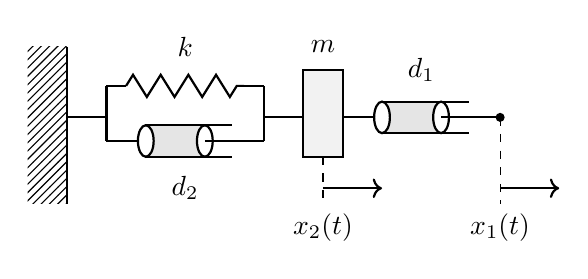
\begin{tikzpicture}[scale=1.0]
          % 固定壁
          \fill[pattern=north east lines] (-1,0,0) rectangle (-0.5,2);
          \draw[thick] (-0.5,0) -- (-0.5,2);
      
          %接続部1
          \draw[thick] (-0.5,1.1) -- (0,1.1);
          \draw[thick] (0,0.8) -- (0,1.5);
        
          % バネ1
          \draw[thick] (0,1.5) -- (0.25,1.5);
          \draw[thick, decorate, decoration={zigzag, segment length=10, amplitude=4}] (0.25,1.5) -- (1.75,1.5);
          \draw[thick] (1.75,1.5) -- (2.0,1.5);
          \node at (1.0,2.0) {$k$};
        
          % ダンパー2(シリンダー形式)
          \draw[thick] (0,0.8) -- (0.5,0.8); % 棒
          \draw[thick, fill=gray!20] (0.5,0.6) rectangle (1.25,1.0); % 筒の側面
          \draw[thick] (1.25,1.0) -- (1.60,1.0); % 筒の上
          \draw[thick] (1.25,0.6) -- (1.60,0.6); % 筒の下
          \draw[thick, fill=white] (0.5,0.8) ellipse (0.1 and 0.2); % 左端面
          \draw[thick, fill=white] (1.25,0.8) ellipse (0.1 and 0.2); % 右端面
          \draw[thick] (1.25,0.8) -- (2.0,0.8); % ピストン棒
          \node at (1.0,0.2) {$d_2$};
      
          %接続部2
          \draw[thick] (2.0,0.8) -- (2.0,1.5);
          \draw[thick] (2.0,1.1) -- (2.5,1.1);
        
          % 質量M
          \draw[thick, fill=gray!10] (2.5,0.6) rectangle (3.0,1.7);
          \node at (2.75,2.0) {$m$};
      
          % ダンパー1(シリンダー形式)
          \draw[thick] (3,1.1) -- (3.5,1.1); % 棒
          \draw[thick, fill=gray!20] (3.5,0.9) rectangle (4.25,1.3); % 筒の側面
          \draw[thick] (4.25,1.3) -- (4.60,1.3); % 筒の上
          \draw[thick] (4.25,0.9) -- (4.60,0.9); % 筒の下
          \draw[thick, fill=white] (3.5,1.1) ellipse (0.1 and 0.2); % 左端面
          \draw[thick, fill=white] (4.25,1.1) ellipse (0.1 and 0.2); % 右端面
          \draw[thick] (4.25,1.1) -- (5,1.1); % ピストン棒
          \node at (4.0,1.7) {$d_1$};
      
          % 丸
          \draw[fill] (5,1.1) circle (0.05);
      
        
          % 座標x1
          \draw[->, thick] (5,0.2) -- (5.75,0.2);
          \node at (5,-0.3) {$x_1(t)$};
          \draw[dashed] (5,1.1) -- (5,0);
      
          % 座標x2
          \draw[->, thick] (2.75,0.2) -- (3.5,0.2);
          \node at (2.75,-0.3) {$x_2(t)$};
          \draw[dashed] (2.75,0.6) -- (2.75,0);
        
        \end{tikzpicture}
    \end{center}
\end{minipage}\\

\indent
(1)この図によって示されるシステムの運動方程式と伝達関数を求めよ。\\

\indent
(2)\(x_1(t)\)に単位ステップ入力を印加した際の応答について、\(x_2(t)\)の定常値を求めよ。\\

\indent
(3)\(m=1,d_1=1,d_2=1,k=1\)としインパルス応答,ステップ応答をそれぞれ求めよ。\\

\indent
(4)\(m=1,d_1=2,d_2=2,k=5\)とし、ステップ応答を求めよ。\\

\indent
(5)\(m=d_1=d_2=k=1\)とし、入力\(x_1(t)=\sin(t)\)を与えたときの応答を求めよ。\\

\indent
(6)\(m=d_1=1,d_2=k=2\)とし、入力\(x_1(t)=\sin(2t)\)を与えたときの応答を求めよ。\\

\indent
(7)\(m=1,d_1=2,d_2=0,k=2\)とし、ステップ応答を求めよ。

% ---------------[5(1)]--------------- 済
\begin{tcolorbox}[title={5. (1)この図によって示されるシステムの運動方程式と伝達関数を求めよ。 
    }]

    \(x(t)\)に関する運動方程式は
    \vspace{-4mm}
    \begin{align*}
        &\qquad m\ddot{x}_2 =-k x_2 - d_2 \dot{x}_2 - d_1 \left(\dot{x}_2 - \dot{x}_1\right) 
    \end{align*}
    \vspace{-4mm}
    また伝達関数は
    \begin{align*}
        &\qquad m\ddot{x}_2 +  (d_1+d_2) \dot{x}_2 + k x_2
        = d_1 \dot{x}_1 \\
        &\therefore \quad \mathcal{L} \left[m\ddot{x}_2 +  (d_1+d_2) \dot{x}_2 + k x_2\right] 
        =\mathcal{L} \left[d_1 \dot{x}_1 \right] \\
        &\therefore \quad \left\{m s^2 +(d_1+d_2) s + k \right\}\,X_2(s) = d_1 s  X_1(s) \quad [\because \dot{x}(0)=x(0)=0 ]\\
        &\therefore \quad G(s) \;=\;\frac{X_2(s)}{X_1(s)}
        \;=\;\frac{d_1 s}{m s^2 +(d_1+d_2) s + k}
    \end{align*}
\end{tcolorbox}

% ---------------[5(2)]--------------- 済
\begin{tcolorbox}[title={5. (2)\(x_1(t)\)に単位ステップ入力を印加した際の応答について、\(x_2(t)\)の定常値を求めよ。 
    }]

            ステップ入力のラプラス変換は\(X_1(s)=\frac{1}{s}\)なので
    \vspace{-4mm}
    \begin{align*}
        &\qquad G(s) = \frac{d_1 s}{m s^2 +(d_1+d_2) s + k} \\
        &\therefore \quad X_o(s) = G(s) X_i(s) = \frac{d_1}{m s^2 +(d_1+d_2) s + k}
    \end{align*}
    最終値定理より
    \vspace{-4mm}
    \begin{align*}
    \lim_{t \to \infty} x_o(t) &= \lim_{s \to 0} sX_o(s) \\
        &= \lim_{s \to 0} \frac{d_1 s}{m s^2 +(d_1+d_2) s + k} \\
        &= 0
    \end{align*}
\end{tcolorbox}

% ---------------[5(3)]--------------- 済
\begin{tcolorbox}[title={5. (3)\(m=1,d_1=1,d_2=1,k=1\)とし、インパルス応答、ステップ応答をそれぞれ\\
\indent \quad 求めよ。}]

(\uppercase\expandafter{\romannumeral 1})インパルス応答 \\
    パラメータを代入し、インパルス入力のラプラス変換は\(F(s)=1\)なので
    \vspace{-2mm}
    \begin{align*}
        &\qquad G(s) = \frac{s}{s^2 + 2 s + 1 } \\
        &\therefore \quad X(s) = G(s) F(s) = \frac{s}{(s+1)^2} \\
        &\therefore \quad X(s) = \frac{-1}{(s+1)^2} + \frac{1}{s+1} \\
        &\therefore \quad \mathcal{L}^{-1} \left[ X(s)\right] 
        =\mathcal{L}^{-1} \left[\frac{-1}{(s+1)^2}\right] 
        + \mathcal{L}^{-1} \left[\frac{1}{s+1}\right] \\
        &\therefore \quad x(t) = - e^{-t} (t-1) 
    \end{align*}

    (\uppercase\expandafter{\romannumeral 2})ステップ応答 \\
    パラメータを代入し、ステップ入力のラプラス変換は\(F(s)=\dfrac{1}{s}\)なので
    \vspace{-2mm}
    \begin{align*}
        &\qquad G(s) = \frac{s}{s^2 + 2 s + 1 } \\
        &\therefore \quad X(s) = G(s) F(s) = \frac{1}{(s+1)^2} \\
        &\therefore \quad \mathcal{L}^{-1} \left[ X(s)\right] 
        =\mathcal{L}^{-1} \left[\frac{1}{(s+1)^2}\right] \\
        &\therefore \quad x(t) = te^{-t} 
    \end{align*}

\end{tcolorbox}

% ---------------[5(4)]--------------- 済
\begin{tcolorbox}[title={5. (4)\(m=1,d_1=2,d_2=2,k=5\)とし、ステップ応答を求めよ。 }]

    パラメータを代入し、ステップ入力のラプラス変換は\(F(s)=\dfrac{1}{s}\)なので
    \vspace{-4mm}
    \begin{align*}
        &\qquad G(s) = \frac{2s}{s^2 + 4s + 5 } \\
        &\therefore \quad X(s) = G(s) F(s) 
        = \frac{2}{(s+2)^2+1^2} \\
        &\therefore \quad \mathcal{L}^{-1} \left[ X(s)\right] 
        = \mathcal{L}^{-1} \left[\frac{2}{(s+2)^2+1^2}\right] \\
        &\therefore \quad x(t) = 2e^{-2t} \sin t
    \end{align*}

\end{tcolorbox}

% ---------------[5(5)]--------------- 済
\begin{tcolorbox}[title={5. (5)\(m=1,d_1=1,d_2=1,k=1\)とし、入力変位\(x_1(t)=\sin(t)\)を与えたときの応
\indent \quad 答を求めよ。 }]

パラメータを代入し、\(x_1(t)=\sin(t)\)のラプラス変換は\(X_i(s)=\dfrac{1}{s^2+1}\)なので
    \vspace{-4mm}
    \begin{align*}
        &\qquad G(s) = \frac{s}{s^2 + 2s + 1} \\
        &\therefore \quad X(s) = G(s) F(s) = \frac{s}{(s+1)^2(s^2 +1)} \\
        &\therefore \quad X(s) =  \frac{\left(-\frac{1}{2}\right)}{(s+1)^2}
        + \frac{\left(\frac{1}{2}\right)}{s^2 +1}\\
        &\therefore \quad \mathcal{L}^{-1} \left[ X(s)\right] 
        = \mathcal{L}^{-1} \left[\frac{\left(-\frac{1}{2}\right)}{(s+1)^2}\right]
        + \mathcal{L}^{-1} \left[\frac{\left(\frac{1}{2}\right)}{s^2 +1}\right] \\
        &\therefore \quad x(t) = -\frac{1}{2} t e^{-t} + \frac{1}{2} \sin t
    \end{align*}

\end{tcolorbox}

% ---------------[5(6)]--------------- 済
\begin{tcolorbox}[title={5. (6)\(m=1,d_1=1,d_2=2,k=2\)とし、入力変位\(x_1(t)=\sin(2t)\)を与えたときの応
\indent \quad 答を求めよ。 }]

パラメータを代入し、\(x_1(t)=\sin(2t)\)のラプラス変換は\(X_i(s)=\dfrac{2}{s^2+2^2}\)なので
    \vspace{-4mm}
    \begin{align*}
        &\qquad G(s) = \frac{s}{s^2 + 3s + 2} \\
        &\therefore \quad X(s) = G(s) F(s) = \frac{s}{(s+1)(s+2)(s^2+2^2)} \\
        &\therefore \quad X(s) =  \frac{\left(-\frac{1}{5}\right)}{s+1} 
        + \frac{\left(\frac{1}{4}\right)}{s+2}
        + \frac{\left(-\frac{1}{20}s+\frac{3}{10}\right)}{s^2+2^2}\\
        &\therefore \quad \mathcal{L}^{-1} \left[ X(s)\right] 
        = \mathcal{L}^{-1} \left[\frac{\left(-\frac{1}{5}\right)}{s+1}  \right]
        + \mathcal{L}^{-1} \left[\frac{\left(\frac{1}{4}\right)}{s+2} \right]
        + \mathcal{L}^{-1} \left[\frac{\left(-\frac{1}{20}s+\frac{3}{10}\right)}{s^2+2^2}\right]  \\
        &\therefore \quad x(t) = -\frac{1}{5} e^{-t} + \frac{1}{4} e^{-2t} - \frac{1}{20} \left\{ \cos (2t) - 3\sin (2t)\right\}
    \end{align*}

\end{tcolorbox}

% ---------------[5(7)]--------------- 済
\begin{tcolorbox}[title={5. (7)\(m=1,d_1=2,d_2=0,k=2\)とし、ステップ応答を求めよ。 }]

    パラメータを代入し、ステップ入力のラプラス変換は\(F(s)=\dfrac{1}{s}\)なので
    \vspace{-4mm}
    \begin{align*}
        &\qquad G(s) = \frac{2s}{s^2 + 2s + 2} \\
        &\therefore \quad X(s) = G(s) F(s) 
        = \frac{2}{s^2 + 2s + 2} \\
        &\therefore \quad \mathcal{L}^{-1} \left[ X(s)\right] 
        = \mathcal{L}^{-1} \left[\frac{2}{(s+1)^2+1}\right] \\
        &\therefore \quad x(t) = 2 e^{-t} \sin t
    \end{align*}

\end{tcolorbox}

% ---------------[6]--------------- 
\begin{tcolorbox}[title={6. 伝達関数\(G_1(s)=\dfrac{1}{s+0.1}\)について漸近線を用いてボード線図を描け。
まず\(10 \times \dfrac{1}{10s+1}\)として一次遅れ系に変形した上で、
ゲイン(dB)、位相(deg.)を求めよ。各軸には適宜数値を記入し、
折れ点等の特徴点を明示すること。}]

\end{tcolorbox}

% ---------------[7]---------------
\begin{tcolorbox}[title={7. \(G(s)=\dfrac{10}{s(s+1)}\)について、周波数応答関数、ゲイン(dB)、位相(deg.)を求めよ。
また、漸近線を用いてボード線図の概形を描け。各軸には適宜数値を記入し、折れ点等の特徴点を明示すること。}]

\end{tcolorbox}

\end{document}